
\documentclass[border=10pt]{standalone}
\usepackage[table]{xcolor}
\usepackage{amsmath,amssymb,amsfonts,mathtools,bm}
\usepackage{booktabs,array}
\usepackage{tikz}
\usetikzlibrary{arrows.meta,positioning,calc,backgrounds,fit,shapes.geometric,decorations.pathreplacing}
\usepackage{pgfplots}
\pgfplotsset{compat=1.18}
\definecolor{sbnavy}{HTML}{1A2A4F}
\definecolor{sbteal}{HTML}{1C7293}
\definecolor{sbaccent}{HTML}{B5651D}
\definecolor{sbgrey}{HTML}{8A94A6}
\definecolor{sblight}{HTML}{EAF1F5}
\newcommand{\cmark}{\textcolor{sbteal}{\ensuremath{\boldsymbol{\checkmark}}}}
\newcommand{\xmark}{\textcolor{sbgrey}{\ensuremath{\boldsymbol{\times}}}}
\newcommand{\eqcol}{\color{sbnavy}}
\begin{document}
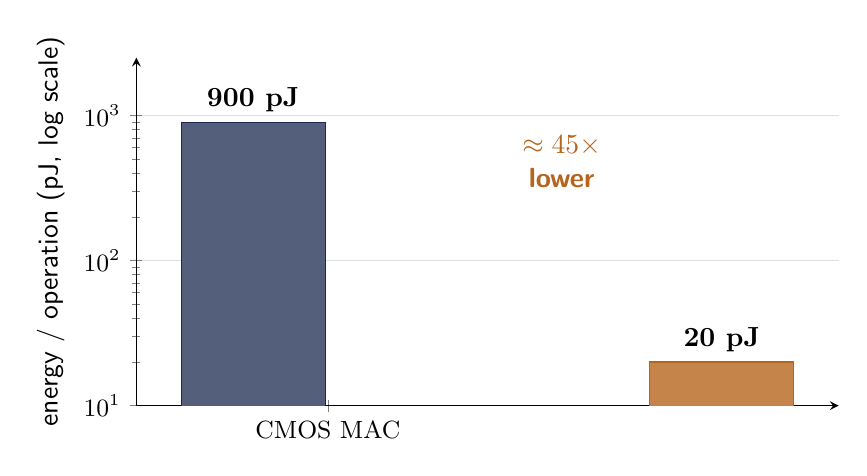
\begin{tikzpicture}
\begin{axis}[
  font=\sffamily, width=10.5cm, height=6cm, ybar, bar width=52pt,
  ymode=log, ymin=10, ymax=2500, ylabel={energy / operation (pJ, log scale)},
  symbolic x coords={CMOS MAC, Neuromorphic}, xtick=data,
  nodes near coords style={font=\bfseries, anchor=south},
  axis lines=left, ymajorgrids, grid style={sbgrey!30},
  enlarge x limits=0.6, tick label style={font=\small}]
  \addplot[draw=sbnavy,fill=sbnavy!75,nodes near coords={900~pJ}] coordinates {(CMOS MAC,900)};
  \addplot[draw=sbaccent,fill=sbaccent!80,nodes near coords={20~pJ}] coordinates {(Neuromorphic,20)};
\end{axis}
\node[font=\sffamily\bfseries,sbaccent,align=center] at (5.4,3.1) {$\approx 45\times$\\ lower};
\end{tikzpicture}
\end{document}